\documentclass{beamer}
%
% Choose how your presentation looks.
%
% For more themes, color themes and font themes, see:
% http://deic.uab.es/~iblanes/beamer_gallery/index_by_theme.html
%
\mode<presentation>
{
  \usetheme{Madrid}      % or try Darmstadt, Madrid, Warsaw, ...
  \usecolortheme{default} % or try albatross, beaver, crane, ...
  \usefonttheme{default}  % or try serif, structurebold, ...
  \setbeamertemplate{navigation symbols}{}
  \setbeamertemplate{caption}[numbered]
}

\usepackage[english]{babel}
\usepackage[utf8x]{inputenc}

\usepackage{listings}
\usepackage{color}

\definecolor{mygreen}{rgb}{0,0.6,0}
\definecolor{mygray}{rgb}{0.5,0.5,0.5}
\definecolor{mymauve}{rgb}{0.58,0,0.82}

\lstset{
  backgroundcolor=\color{white},   % choose the background color; you must add \usepackage{color} or \usepackage{xcolor}; should come as last argument
  basicstyle=\footnotesize,        % the size of the fonts that are used for the code
  breakatwhitespace=false,         % sets if automatic breaks should only happen at whitespace
  breaklines=true,                 % sets automatic line breaking
  captionpos=b,                    % sets the caption-position to bottom
  commentstyle=\color{mygreen},    % comment style
  deletekeywords={...},            % if you want to delete keywords from the given language
  escapeinside={\%*}{*)},          % if you want to add LaTeX within your code
  extendedchars=true,              % lets you use non-ASCII characters; for 8-bits encodings only, does not work with UTF-8
  frame=single,	                   % adds a frame around the code
  keepspaces=true,                 % keeps spaces in text, useful for keeping indentation of code (possibly needs columns=flexible)
  keywordstyle=\color{blue},       % keyword style
  language=C++,                    % the language of the code
  morekeywords={*,...},            % if you want to add more keywords to the set
  %numbers=left,                    % where to put the line-numbers; possible values are (none, left, right)
  %numbersep=5pt,                   % how far the line-numbers are from the code
  %numberstyle=\tiny\color{mygray}, % the style that is used for the line-numbers
  rulecolor=\color{black},         % if not set, the frame-color may be changed on line-breaks within not-black text (e.g. comments (green here))
  showspaces=false,                % show spaces everywhere adding particular underscores; it overrides 'showstringspaces'
  showstringspaces=false,          % underline spaces within strings only
  showtabs=false,                  % show tabs within strings adding particular underscores
  stepnumber=2,                    % the step between two line-numbers. If it's 1, each line will be numbered
  stringstyle=\color{mymauve},     % string literal style
  tabsize=2,	                   % sets default tabsize to 2 spaces
  title=\lstname                   % show the filename of files included with \lstinputlisting; also try caption instead of title
}


\title[Programaci\'on din\'amica]{Programaci\'on din\'amica}
%\author{You}
%\institute{}
%\date{Date of Presentation}

\begin{document}

\begin{frame}
  \titlepage
\end{frame}

% Uncomment these lines for an automatically generated outline.
\begin{frame}{Contenidos}
  \tableofcontents
\end{frame}

\section{Programaci\'on din\'amica}

\subsection{Sucesi\'on de Fibonacci}

\begin{frame}[fragile]{Sucesi\'on de Fibonacci}
\begin{block}{Definici\'on}
La sucesi\'on de Fibonacci se define como $fib_0 = 0, fib_1 = 1$, $fib_n = fib_{n-1} + fib_{n-2}$ (para $n \ge 2$). Los primeros t\'erminos son $0,1,1,2,3,5,8,13,21 ...$
\end{block}
\begin{itemize}
\item
La definici\'on nos sugiere una forma de computarlo (funci\'on recursiva).
\end{itemize}
\begin{columns}
\begin{column}{0.5\textwidth}
\begin{lstlisting}
int fib(int n){
	if(n <= 1)
		return n;
	return fib(n-1) + fib(n-2);
}
\end{lstlisting}
\end{column}
\begin{column}{0.5\textwidth}
\pause
Notemos que este programa es ineficiente porque calcula muchas veces lo mismo (por ejemplo, fib(n-2) se calcula en fib(n) y tambi\'en en la llamada recursiva a fib(n-1).
\end{column}
\end{columns}
\end{frame}

\begin{frame}{Fibonacci (cont.)}
\begin{figure}
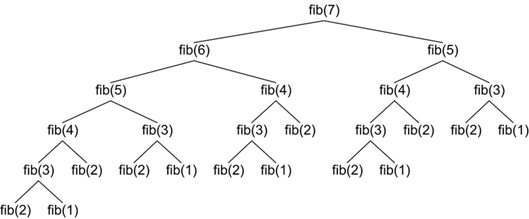
\includegraphics[width=\textwidth]{fibo}
\end{figure}
\begin{itemize}
\item
La complejidad es exponencial en n.
\end{itemize}
\end{frame}
\begin{frame}[fragile]{Fibonacci - din\'amica}
\begin{itemize}
\item
Podemos hacerlo mejor: en lugar de recalcular la respuesta cada vez, la calculamos una sola vez y guardamos el resultado.
\end{itemize}
\begin{columns}
\begin{column}{0.5\textwidth}
\begin{lstlisting}
int mem[MAX_N];
int fib(int n){
	if(mem[n] >= 0)
		return mem[n]
	int res;
	if(n <= 1)
		res = n;
	else
		res = fib(n-1) + fib(n-2);
	mem[n] = res;
	return res;
}
// (al principio de main):
	fill(mem, mem+MAX_N, -1);
\end{lstlisting}
\end{column}
\begin{column}{0.5\textwidth}
\begin{itemize}
\item
En el arreglo mem guardamos los resultados para los n's que ya calculamos (usamos un valor negativo para indicar que no lo calculamos).
\item
Ahora la complejidad de calcular todos los fibonaccis hasta $n$ es $O(n)$ .
\end{itemize}
\end{column}
\end{columns}
\end{frame}

\subsection{Definici\'on de programaci\'on din\'amica}

\begin{frame}{Programaci\'on din\'amica - definici\'on}
\begin{itemize}
\item
La programaci\'on din\'amica es, b\'asicamente, una recursi\'on con una especie de cach\'e para guardar resultados ya calculados.
\item
Podemos verla como un m\'etodo para resolver un problema, que lo parte en subproblemas m\'as peque\~nos, los cu\'ales resuelve recursivamente, guardando los resultados para no calcularlos m\'as de una vez.
\item
En el contexto de programaci\'on din\'amica, llamamos ``estado'' a cada combinaci\'on de par\'ametros de la misma. En el caso de Fibonacci, el estado es el valor de $n$.
\item
Para calcular el costo de la programaci\'on din\'amica, la cuenta suele ser ``cantidad de estados'' * ``costo de calcular el valor de un estado (sin contar las llamadas recursivas)''

\end{itemize}
\end{frame}

\subsection{Versi\'on iterativa vs. recursiva}

\begin{frame}[fragile]{Fibonacci - versi\'on iterativa}
\begin{lstlisting}
int fib[MAXN];
void calcFibs(int n){
//	calcula todos los fibonaccis hasta n
//	y los guarda en el arreglo fib
	fib[0] = 0;
	fib[1] = 1;
	for(int i = 2; i <= n; ++i)
		fib[i] = fib[i-1] + fib[i-2];
}
\end{lstlisting}

\begin{itemize}
\item
Todo problema de programaci\'on din\'amica se puede resolver recursivamente (c\'omo se mostr\'o antes) o iterativamente.
\item
La forma recursiva se suele llamar ``memoizaci\'on'' (\textit{memoization} en ingl\'es).
\end{itemize}

\end{frame}

\begin{frame}{Progamaci\'on din\'amica iterativa vs. recursiva}
\begin{itemize}
\item
Tanto la forma iterativa como la recursiva tienen ventajas y desventajas.
\item
Forma iterativa:
\begin{itemize}
\item
Suele ser m\'as eficiente en tiempo, porque se evitan las llamadas a funci\'on.
\item
A veces permite ahorrar memoria (lo veremos m\'as adelante).
\item
El c\'odigo suele resultar m\'as corto.
\end{itemize}
\item
Forma recursiva:
\begin{itemize}
\item
Para muchos es el modo m\'as ``natural'' de pensar la programaci\'on din\'amica.
\item
No requiere pensar en el orden en el que debemos calcular los sub-problemas, que no siempre es obvio.
\item
Es m\'as eficiente cuando hay muchos valores de la tabla que no es necesario calcular (no es muy com\'un, pero puede ocurrir).
\end{itemize}
\end{itemize}
\end{frame}

\section{N\'umeros combinatorios}

\begin{frame}{N\'umeros combinatorios}
\begin{block}{Definici\'on}
El n\'umero combinatorio $\binom{n}{k}$ se define como la cantidad de formas de elegir $k$ elementos distintos de un conjunto de tama\~no n.
\end{block}
\begin{itemize}
\item
Identifiquemos los elementos con los n\'umeros del $1$ al $n$.
\item
Si $n \ge 1$, tenemos dos opciones: tomamos el elemento $n$ y elegimos $k-1$ elementos de los $n-1$ restantes, o no tomamos el $n$-\'esimo y elegimos $k$ elementos de los $n-1$ restantes.
\item
Luego, tenemos la recurrencia $\binom{n}{k} = \binom{n-1}{k-1} + \binom{n-1}{k}$.
\item
!`Podemos usar programaci\'on din\'amica! Los casos bases ser\'ian $\binom{n}{0} = 1$, $\binom{n}{k} = 0$ para $k > n$.
\end{itemize}
\end{frame}

\begin{frame}[fragile]{Combinatorios - c\'odigo recursivo}
\begin{lstlisting}
int mem[MAXN][MAXN];
int comb(int n, int k){
//	precondicion: mem esta inicializado en -1
	if(mem[n][k] >= 0)
		return mem[n][k];
	int res;
	if(k == 0)
		res = 1;
	else if(k > n)
		res = 0;
	else
		res = comb(n-1, k-1) + comb(n-1, k);
	mem[n][k] = res;
	return res;
}
\end{lstlisting}
\end{frame}

\begin{frame}[fragile]{Combinatorios - c\'odigo iterativo}
\begin{lstlisting}
int comb[MAXN][MAXN];
void calcCombs(){
//	precondicion: comb esta inicializado en 0
	for(int i = 0; i < MAXN; ++i){
    	comb[i][0] = comb[i][i] = 1;
        for(int j = 1; j < i; ++j)
        	comb[i][j] = comb[i-1][j-1] + comb[i-1][j];
    }
}
\end{lstlisting}
\begin{itemize}
\item
Esta tabla se conoce com\'unmente como ``Tri\'angulo de Pascal''
\item
La complejidad de ambas versiones es $O(MAXN^2)$
\end{itemize}
\end{frame}
\begin{frame}{Combinatorios - cont.}
\begin{itemize}
\item
Notemos que los n\'umeros combinatorios tambi\'en se pueden calcular mediante la f\'ormula $\frac{n!}{k!(n-k)!}$. Sin embargo, la recurrencia es m\'as eficiente cuando se quieren calcular muchos valores, y $n$ no es muy grande.
\item
Los n\'umeros combinatorios aparecen en muchos problemas de conteo y probabilidad. Es \'util saber implementar r\'apido la versi\'on iterativa de la tabla.
\end{itemize}
\end{frame}

\section{Problema de la moneda}

\begin{frame}{Problemas de optimizaci\'on}
\begin{itemize}
\item
La programaci\'on din\'amica se puede usar tambi\'en para resolver algunos problemas de optimizaci\'on (encontrar la mejor soluci\'on, de acuerdo a cierto criterio).
\item
?`Se acuerdan del problema de la moneda? (el que vimos en su versi\'on greedy). En el caso general se puede resolver con programaci\'on din\'amica.
\end{itemize}
\end{frame}

\begin{frame}{Problema de la moneda}
\begin{block}{Enunciado}
Tenemos $n$ tipos de monedas de valores $v_0,v_1,...,v_{n-1}$. \\
Queremos saber la menor cantidad de monedas que necesitamos para sumar exactamente $m$.
\end{block}
\begin{itemize}
\item
Definimos $f(k,j) = $ ``menor cantidad de monedas que necesitamos para sumar exactamente $j$ usando s\'olo los primeros $k$ valores de monedas ($v_0,...,v_{k-1}$)''. Nos interesa calcular $f(n,m)$.
\item
Si $k \ge 1$ consideramos dos opciones:
\begin{itemize}
\item
No usamos la moneda de valor $v_{k-1}$. Esto es lo mismo que resolver el subproblema para $(k-1,j)$.
\item
Usamos la moneda de valor $v_{k-1}$ al menos una vez. Esto es lo mismo que resolver el subproblema para $(k,j-v_{k-1})$ y agregar una moneda de valor $v_{k-1}$.
\end{itemize}
\item
Esto nos da la recurrencia: $f(k,j) = min(f(k-1,j), 1+f(k,j-v_{k-1}))$.
\end{itemize}
\end{frame}

\subsection{Recurrencia}

\begin{frame}{Problema de la moneda - recurrencia}
Agregando los casos bases, queda:
\[
    f(k,j)=
\begin{cases}
    0,& \text{si } k=0 \text{ y } j=0\\
    \infty,& \text{si } (k=0 \text{ y } j \neq 0) \text{ \'o } j < 0\\
    min(f(k-1,j), 1+f(k,j-v_{k-1})), & \text{caso contrario}\\
\end{cases}
\]
\begin{itemize}
\item
Como lo que queremos es un m\'inimo, el valor $\infty$ representa la ausencia de soluci\'on. A nivel c\'odigo, se puede usar un valor lo suficientemente alto, de modo que nunca una soluci\'on pueda tener ese tama\~no.
\item
La complejidad es $O(n*m)$
\end{itemize}
\end{frame}

\begin{frame}[fragile]{Problema de la moneda - C\'odigo recursivo}
\begin{lstlisting}
int v[MAXN];
int mem[MAXN][MAXM];
int f(int k, int j){
//	precondicion: mem esta inicializado en -1
	if(j < 0)
		return INF;
	if(mem[k][j] >= 0)
		return mem[n][k];
	int res;
	if(k == 0){
		if(j == 0)
	    	res = 0;
	    else
	    	res = INF;
	}
	else
		res = min(f(k-1,j),1+f(k,j-v[k-1]));
	mem[k][j] = res;
	return res;
}
\end{lstlisting}
\end{frame}

\begin{frame}[fragile]{Problema de la moneda - C\'odigo iterativo}
\begin{lstlisting}
int v[MAXN];
int f[MAXN][MAXM];
int solve(int n, int m){
	f[0][0] = 0;
	for(int j = 1; j <= m; ++j)
		f[0][j] = INF;
	for(int k = 1; k <= n; ++k){
		for(int j = 0; j <= m; ++j){
			f[k][j] = f[k-1][j];
			if(v[k-1] <= j)
				f[k][j]=min(f[k][j],1+f[k][j-v[k-1]]);
		}
	}
	return f[n][m];
}
\end{lstlisting}
\end{frame}

\subsection{Generar soluci\'on \'optima}

\begin{frame}{Moneda - Generar soluci\'on}
\begin{itemize}
\item
En muchos problemas de optimizaci\'on, adem\'as del valor de la soluci\'on \'optima, se nos pide que demos expl\'icitamente la soluci\'on (en el caso de moneda, cu\'antas monedas tengo que tomar de cada tipo).
\item
Podemos aprovechar que tenemos guardado el resultado de todos los sub-problemas.
\item
Empezamos desde el estado $(n,m)$
\begin{itemize}
\item
Si $f(n,m)=f(n-1,m)$ recursionamos para $(n-1,m)$.
\item
Si no, es porque tenemos que agregar la moneda $n-1$. La agregamos al resultado y recursionamos para $(n,m-v_{n-1})$.
\item
Seguimos hasta llegar a $(0,0)$.
\end{itemize}

\end{itemize}
\end{frame}

\begin{frame}[fragile]{Mondeda - C\'odigo para generar soluci\'on}
\begin{lstlisting}
int f[MAXN][MAXM];
int sol[MAXN];
void gen_rec(int k, int j){
	if(k == 0)
		return;
	if(f[k][j] == f[k-1][j])
		gen_rec(k-1, j);
	else {
		sol[k-1]++;
		gen_rec(k, j - v[k][j-v[k-1]]);
	}
}
void generate(int n, int m){
//	guarda en sol cuantas monedas necesito para cada valor
//	precondicion: f contiene los resultados para cada subproblema
	fill(sol, sol+n, 0);
	gen_rec(n,m)
}
\end{lstlisting}
\end{frame}
\begin{frame}{Generar soluci\'on}
\begin{itemize}
\item
Este patr\'on para generar una soluci\'on \'optima se puede aplicar a cualquier programaci\'on din\'amica que resuelva un problema de optimizaci\'on.
\item
Partimos del estado que nos interesa.
\item
En cada paso usamos los valores calculados para ver qu\'e decisi\'on coincide con el resultado del estado.
\item
Guardamos en la soluci\'on la decisi\'on que tomamos (en el caso de moneda, incrementamos la cantidad de monedas del valor que consideramos en el caso de que nos conviene).
\item
Recursionamos para los sub-problemas.
\end{itemize}
\end{frame}

\subsection{Contar soluciones \'optimas}

\begin{frame}{Moneda - Contar soluciones \'optimas}
\begin{itemize}
\item
?`Qu\'e pasa si adem\'as se nos pide la cantidad de soluciones \'optimas?
\item
Resulta que tambi\'en podemos aplicar programaci\'on din\'amica para contar la cantidad de soluciones mientras calculamos el valor \'optimo.
\item
La recurrencia es como sigue:
\begin{itemize}
\item
En el caso base ($k=0$) hay una s\'ola soluci\'on (no poner nada).
\item
Si $k>0$ y da lo mismo tomar la moneda $k-1$ que no tomarla ($f(k-1,j) = 1 + f(k,j-v_{k-1})$), sumamos la cantidad de soluciones de los subproblemas  $(k-1,j)$ y $(k,j-v_{k-1})$.
\item
Si una de las dos opciones es estrictamente mejor que la otra, la cantidad de soluciones es igual a la cantidad de soluciones del subproblema correspondiente.
\end{itemize}
\item
Esta t\'ecnica para contar soluciones se puede adaptar a cualquier programaci\'on din\'amica de optimizaci\'on.
\end{itemize}
\end{frame}

\begin{frame}[fragile]{Contar soluciones \'optimas - C\'odigo iterativo}
\begin{lstlisting}
int v[MAXN],f[MAXN][MAXM];
int cnt[MAXN][MAXM]; // tabla para cantidad de soluciones
pair<int,int> solve(int n, int m){
//	devuelve un par (valor optimo, cantidad de soluciones)
	f[0][0] = 0; cnt[0][0] = 1;
	fill(f[0]+1,f[0]+m+1,INF);
	for(int k = 1; k <= n; ++k)
		for(int j = 0; j <= m; ++j){
			f[k][j] = f[k-1][j]; cnt[k][j] = cnt[k-1][j];
			if(v[k-1] <= j){
				if(1+f[k][j-v[k-1]] < f[k][j]){
					f[k][j] = 1+f[k][j-v[k-1]];
					cnt[k][j] = cnt[k][j-v[k-1]];
				}
				else if(1+f[k][j-v[k-1]] == f[k][j])
					cnt[k][j] += cnt[k][j-v[k-1]];
			}
		}
	return {f[n][m],cnt[n][m]};
}

\end{lstlisting}
\end{frame}

\subsection{Optimizaci\'on de memoria}

\begin{frame}[fragile]{Moneda - optimizaci\'on de memoria}
\begin{itemize}
\item
Para el problema de la moneda (y muchos otros donde una de las variables del estado solo puede decrecer en uno en la transici\'on) podemos ahorrar memoria haci\'endolo de forma iterativa.
\item
Si bien la complejidad es la misma, tener menos memoria reduce el tiempo de ejecuci\'on porque disminuye los fallos de cach\'e.
\item
Algunos problemas requieren esta optimizaci\'on para entrar en los l\'imites de tiempo y memoria.
\end{itemize}
\begin{columns}
\begin{column}{0.65\textwidth}
\begin{lstlisting}
int v[MAXN],f[MAXM];
int solve(int n, int m){
	f[0] = 0;
	fill(f+1, f+m+1, INF);
	for(int k = 0; k < n; ++k)
		for(int j = v[k]; j <= m; ++j)
			f[j] = min(f[j], 1 + f[j-v[k]]);
	return f[m];
}
\end{lstlisting}
\end{column}
\begin{column}{0.35\textwidth}
Desventaja: no nos permite reconstruir la soluci\'on.
\end{column}
\end{columns}
\end{frame}

\section{Sumas parciales (1D y 2D)}

\begin{frame}{Sumas parciales - 1D}
\begin{block}{Enunciado}
Dado un arreglo de n\'umeros $a_0...a_{n-1}$. Definimos $sum(l,r) = $ ``suma del sub-arreglo $a_l...a_{r-1}$''. Dadas $q$ pares $(l_i,r_i)$, queremos calcular $sum(l_i,r_i)$ para cada uno.
\end{block}
\begin{itemize}
\item
La soluci\'on m\'as obvia es recorrer el sub-arreglo correspondiente para cada pregunta, calculando la suma en $O(n)$.
\item
Podemos hacerlo mejor observando que $sum(l,r) = sum(0,r) - sum(0,l)$
\item
Luego, si precalculamos $sum(0,i)$ para todo $i$, podemos responder cada pregunta en $O(1)$.
\item
La recurrencia es simple:
\begin{itemize}
\item
$sum(0,0) = 0$
\item
$sum(0,i+1) = sum(0,i) + a_{i}$.
\end{itemize}
\end{itemize}
\end{frame}
\begin{frame}[fragile]{Sumas parciales - 1D - C\'odigo}
\begin{lstlisting}
int a[MAXN],sp[MAXN+1];int n;
void init_sum(){
	sp[0] = 0;
	for(int i = 0; i < n; ++i)
		sp[i+1] = sp[i] + a[i];
}
int sum(int l, int r){
	return sp[r] - sp[l];
}
\end{lstlisting}
\begin{itemize}
\item
La idea de hacer sumas parciales aparece en muchos problemas, es bueno tenerla presente.
\item
Hay otros tipos de estructuras (que se ver\'an m\'as adelante) que permiten adem\'as modificar los valores de $a$ o calcular otro tipo de operaciones sobre intervalos (ej: el m\'inimo).

\end{itemize}
\end{frame}

\begin{frame}{Sumas parciales - 2D}
\begin{block}{Enunciado}
Ahora, queremos resolver el mismo problema, pero en dos dimensiones. Es decir, en vez de tener un arreglo tenemos una matriz, y en vez de calcular la suma de un intervalo queremos calcular la suma de un ``rect\'angulo'' de la matriz. Concretamente, tenemos una matriz $a_{i,j}$ $(i \in [0,n), j \in [0,m))$ y queremos calcular $$sum(i_0,i_1,j_0,j_1) = \sum_{i=i_0}^{i_1-1}\sum_{j=j_0}^{j_1-1} a_{i,j}$$
\end{block}
\begin{itemize}
\item
Podemos aplicar una idea similar al caso de una dimensi\'on.
\end{itemize}
\end{frame}

\begin{frame}{Sumas parciales - 2D - cont.}
\begin{itemize}
\item
Definimos $sp(i,j) = sum(0,i,0,j)$ (suma del rect\'angulo entre $(0,0)$ y $(i-1,j-1)$).
\item
Tenemos que $sum(i_0,i_1,j_0,j_1) = sp(i_1,j_1)-sp(i_1,j_0)-sp(i_0,j_1)+sp(i_0,j_0)$.\\
(dibujito en pizarr\'on).
\item
Entonces, podemos responder en $O(1)$ si precalculamos $sp(i,j)$.
\item
Tenemos que (para $i>0,j>0$) $sp(i,j) = sp(i,j-1)+sp(i-1,j)+a_{i-1,j-1}-sp(i-1,j-1)$.\\
(dibujito en pizarr\'on).
\item
Podemos usar programaci\'on din\'amica para calcular esta recurrencia.
\item
C\'odigo: ejercicio.
\end{itemize}
\end{frame}

\section{Edit distance}

\begin{frame}{Edit distance}
\url{http://www.spoj.com/problems/EDIST/}
\begin{block}{Enunciado}
Dados dos strings $A$ y $B$, decir la menor cantidad de operaciones necesarias para transformar $A$ en $B$. Las operaciones permitidas son:
\begin{itemize}
\item
Agregar un caracter en cualquier posici\'on.
\item
Borrar un caracter.
\item
Cambiar un caracter.
\end{itemize}
Por ejemplo, si $A =$ ``saturday'', $B =$ ``sundays'' una soluci\'on es:\\
``saturday'' $\rightarrow$ ``sturday'' $\rightarrow$ ``surday''  $\rightarrow$ ``sunday'' $\rightarrow$ ``sundays''.
\end{block}
\begin{itemize}
\item
Llamemos $f(A,B)$ al resultado.
\item
Los casos en que $A$ \'o $B$ son vac\'ios son f\'aciles ($f("",B) = |B|$, $f(A,"") = |A|$).
\end{itemize}
\end{frame}
\begin{frame}{Edit distance (cont.)}
\begin{itemize}
\item
Si $A$ y $B$ no son vac\'ios, entonces $A = A'a$, $B = B'b$ (llamamos $a$ y $b$ al \'ultimo caracter de $A$ y $B$ respectivamente).
\item
Si $a = b$, es claro que $f(A,B) = f(A',B')$.
\item
Si $a \neq b$, entonces tenemos que realizar operaciones sobre $A$ para que su \'ultimo caracter sea $b$. Tenemos varias opciones:
\begin{itemize}
\item
Agregamos el caracter $b$ al final de $A$ y resolvemos para $(A,B')$
\item
Borramos el \'ultimo caracter $a$ y resolvemos para $(A',B)$.
\item
Cambiamos el \'ultimo caracter de $A$ por $b$ y resolvemos para $(A',B')$.
\end{itemize}
\item
Es f\'acil convencerse de que este m\'etodo contempla todas las posibilidades \'optimas.
\item
Con estas observaciones, es simple armar una recurrencia sobre $(i,j)$ que calcule ``menor costo de transformar los primeros $i$ caracteres de $A$ en los primeros $j$ caracteres de $B$''.
\item
La recurrencia y el c\'odigo quedan como ejercicio.
\end{itemize}
\end{frame}

\section{Conclusi\'on}

\begin{frame}{Conclusi\'on}
\begin{itemize}
\item
Programaci\'on din\'amica es uno de los t\'opicos m\'as comunes en el contexto de programaci\'on competitiva, por lo que es muy importante dedicarle tiempo a practicarlo.
\item
Si lo permite el cronograma, en una clase posterior veremos cosas m\'as avanzadas acerca de programaci\'on din\'amica (algunos patrones que suelen aparecer, t\'ecnicas de optimizaci\'on).
\item
Un concepto muy relacionado a programaci\'on din\'amica del cual no hablamos es ``backtracking''. Es lo mismo que programaci\'on din\'amica, pero sin guardar informaci\'on de los sub-problemas resueltos (s\'olo la recursi\'on que prueba todas las posibilidades). Se usa backtracking cuando la estructura del problema es tal que cada sub-problema se resuelve una s\'ola vez.
\end{itemize}
\end{frame}

\end{document}

